\subsection{Ca sử dụng tạo lịch trình cho chuyến đi}
\vspace{0.5cm}


\noindent 
\begin{tabularx}{\linewidth}{| l | X |} 
    \hline 
    \textbf{Mô tả} & Người dùng có thể tạo một lịch trình cụ thể cho chuyến đi của mình. \\ 
    \hline 
    \textbf{Luồng cơ bản} & 1. Người dùng chọn một chuyến đi. \newline
                            2. Hệ thống lây dữ liệu chi tiết và hiển thị. \newline
                            3. Người dùng bấm "Thêm lịch trình". \newline
                            4. Hệ thống hiển thị 2 lựa chọn tạo lịch trình. \newline
                            5. Người dùng chọn tùy chọn "chọn từ mục lưu". \newline
                            6. Hệ thống truy xuất và hiển thị các mục lưu của chuyến đí cho người dùng chọn. \newline
                            7. Người dùng chọn mục thêm vào lịch trình. \newline
                            8. Hệ thống hiện thị form điền thông tin lịch trình. \newline
                            9. Người dùng điền thông tin lịch trình như thời gian bắt đầu, ghi chú,v.v. \newline
                            10. Người dùng bấm "Lưu lịch trình". \newline
                            11. Hệ thống lưu lịch trình vào cơ sở dữ liệu và thông báo thành công. \\
                   
    \hline 
    \textbf{Luồng thay thế} & Người dùng chọn tùy chọn "chọn trên bản đồ". \newline
                                1. Hệ thống hiển thị bản đồ. \newline
                                2. Người dùng chọn 1 vị tri trên bản đồ. \newline
                                3. Tiếp tục từ bước 8 của Luồng cơ bản. \\
    
           
    \hline 
    \textbf{Tiền điều kiện} & - Người dùng đang đăng nhập và phiên đăng nhập chưa kết thúc.\newline
    - Người dùng đã tạo hoặc tham gia ít nhất một chuyến đi. \newline
    - Trạng thái chuyến đi khác "Đã hoàn thành" và "Hủy". \\
    \hline 
    \textbf{Hậu điều kiện} & - Hệ thống lưu lịch trình vào cơ sở dữ liệu.\newline
                            - Người dùng có thể chinh sửa lịch trình đã tạo. \newline
                            - Người dùng có thể xem bản đồ trực quan lịch trình đã tạo. \\
    
    \hline 
    \textbf{Yêu cầu phi chức năng} & Hệ thống thêm mục lưu dưới 2s \\ 
    \hline 
    \end{tabularx}


\noindent 
\begin{tabular}{| c | c |}
    \hline
    \textbf{Biểu đồ hoạt động} & \textbf{Quan hệ} \\ 
    \hline
    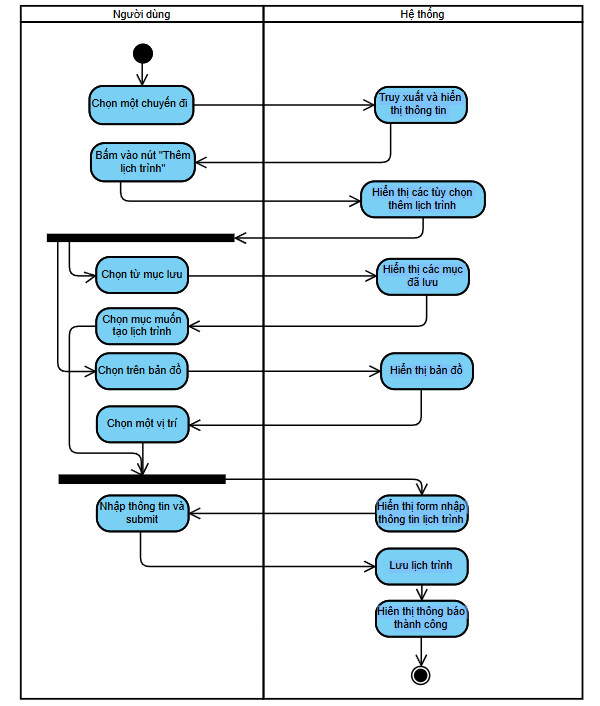
\includegraphics[width=0.5\linewidth]{figures/c3/3-3-13-ad.png} 
    & 
    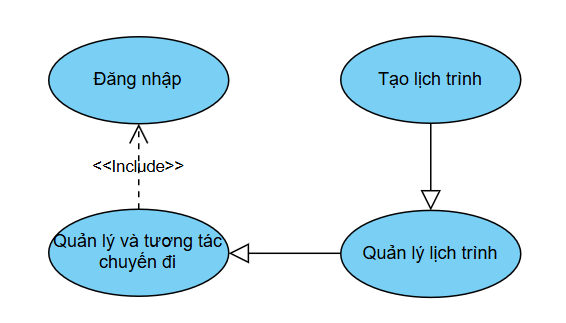
\includegraphics[width=0.45\linewidth]{figures/c3/3-3-13-rd.png} \\ 
    \hline
\end{tabular}


\begin{figure}[H]
    \centering  
    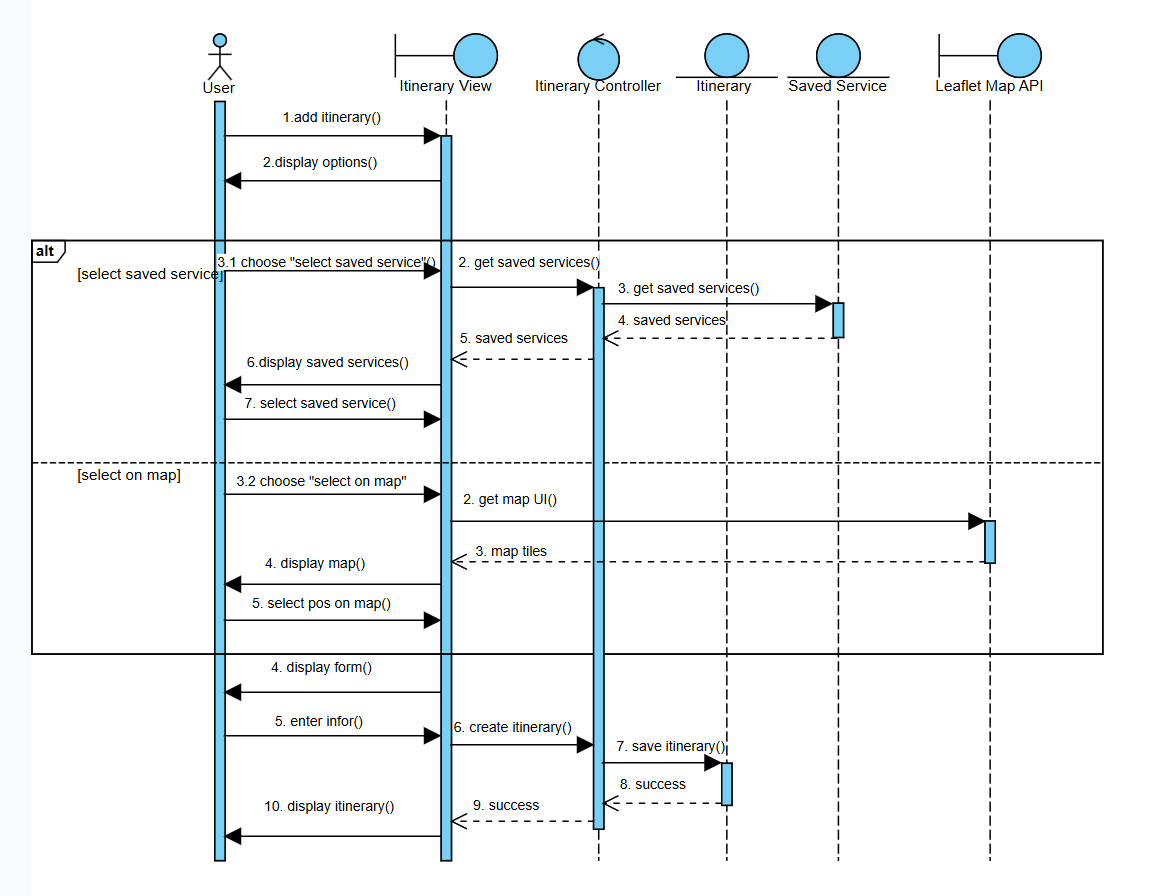
\includegraphics[width=1\textwidth]{figures/c3/3-3-13-sd.png}
    \caption{Biểu đồ tuần tự ca sử dụng tạo lịch trình cho chuyến đi.}
    \label{fig:3-3-13-sequence-diagram}
\end{figure}